\noindent\textbf{Resumen.} Esta parte trabaja sobre los 5.702.270 contratos de plata. Los nulos se dejan sin imputar, los valores imposibles se separan de los atípicos, se exploran los datos, se agrupan 2.603 entidades con K-means y se usa Apriori para ver qué alertas coinciden. Salieron cuatro perfiles de entidades que se mantienen al cambiar la semilla, y las alertas poco comunes tienden a aparecer juntas. Todo esto sirve para ordenar la revisión y no dice nada sobre la conducta de una entidad.

% =============================================================================
\subsection{Introducción}
% =============================================================================
Nadie puede revisar a mano 5,7 millones de contratos para ver qué entidades contratan de forma rara. Contratar sin competencia, firmar un domingo o empezar a ejecutar antes de firmar no prueba nada por sí solo, pero sirve para decidir qué mirar primero~\cite{ocp2016,fazekas2020}. La Sección~\ref{sec:intro} presenta los objetivos y el ODS~16.

La materia atacó dos preguntas. La primera es de calidad: cómo tratar los nulos y los valores imposibles sin perder información. La segunda es de patrones: si hay grupos de entidades con alertas parecidas y qué alertas suelen darse en el mismo contrato.

El conjunto completo nunca se descarga al computador. Athena hace los cálculos en AWS y devuelve resúmenes y una muestra del 0,9~\%.

% =============================================================================
\subsection{Preparación de los datos}
% =============================================================================
\subsubsection{Conjunto limpio}
\label{mineria:sec:limpieza}
Plata conserva 16 de las 91 columnas, limpias con las reglas de la Tabla~\ref{adq:t2}. Al 13 de noviembre de 2026 tiene 5.702.270 contratos, ninguno repetido ni con valor negativo, y todas las fechas de firma caen entre junio de 2015 y noviembre de 2026.

\subsubsection{Nulos}
Ningún nulo se rellena, porque una fecha o un contratista inventados harían aparecer o desaparecer alertas. Once columnas están completas, y las otras cinco reciben el tratamiento de la Tabla~\ref{mineria:tab:nulos}. Que falte el documento del contratista ya es una alerta: sin él no se sabe a quién se le pagó.

\begin{table}[!htbp]
\centering
\caption{Columnas con datos faltantes y qué se hace con ellos}
\label{mineria:tab:nulos}
\footnotesize
\setlength{\tabcolsep}{3pt}
\begin{tabularx}{\columnwidth}{@{}>{\raggedright\arraybackslash}p{0.33\columnwidth}rrL@{}}
\toprule
Campo & Vacíos & \% & Decisión \\
\midrule
\code{codigo\_unspsc} & 181.448 & 3,18 & Se conserva; en fraccionamiento se agrupan juntos \\
\code{fecha\_inicio} & 124.783 & 2,19 & Sin dato, sin alerta de inicio ni de adiciones \\
\code{fecha\_firma} & 63.859 & 1,12 & Fuera de las series; sí cuenta por entidad \\
\code{documento\_\allowbreak proveedor} & 16.220 & 0,28 & Alerta de contratista no identificado \\
\code{fecha\_fin} & 43 & 0,00 & Sin alerta de adiciones \\
\bottomrule
\end{tabularx}
\end{table}

\subsubsection{Valores extremos}
\label{mineria:sec:outliers}
Unos pocos contratos enormes estiran la distribución del valor: su asimetría es 60,7, y baja a 0,24 al tomar $\log_{10}$, que es la escala que se usa en el análisis. Para los valores extremos hay dos reglas con propósitos distintos.

La primera es de calidad. Un solo contrato de más de un billón de COP es casi siempre un error al digitar el valor; hay 85 casos, que siguen en la tabla pero no entran en las sumas. La segunda es estadística y sigue a Tukey~\cite{tukey1977}: un contrato es atípico cuando supera $Q_3+3\,\mathrm{IQR}$ de su mismo tipo de contrato, para no comparar una obra con una prestación de servicios. Así quedan marcados 237.446 contratos, el 4,16~\% (Tabla~\ref{mineria:tab:outliers} y Fig.~\ref{mineria:fig:box}), que se conservan como la alerta de valor atípico.

\begin{table}[!htbp]
\centering
\caption{Desde qué valor un contrato es atípico en su tipo (millones de COP)}
\label{mineria:tab:outliers}
\footnotesize
\begin{tabular}{@{}lrrrr@{}}
\toprule
Tipo & Contratos & Mediana & Umbral & Atípicos \\
\midrule
Servicios & 4.894.743 & 18,7 & 113,7 & 155.564 \\
Otro & 205.545 & 143,2 & 2.404,0 & 17.135 \\
Decreto 092 de 2017 & 204.340 & 15,1 & 184,2 & 24.356 \\
Suministros & 137.738 & 37,6 & 394,0 & 13.613 \\
Compraventa & 111.031 & 28,3 & 317,3 & 11.442 \\
Obra & 50.397 & 216,8 & 3.375,6 & 5.403 \\
\bottomrule
\end{tabular}
\end{table}

\begin{figure}[!htbp]
\centering



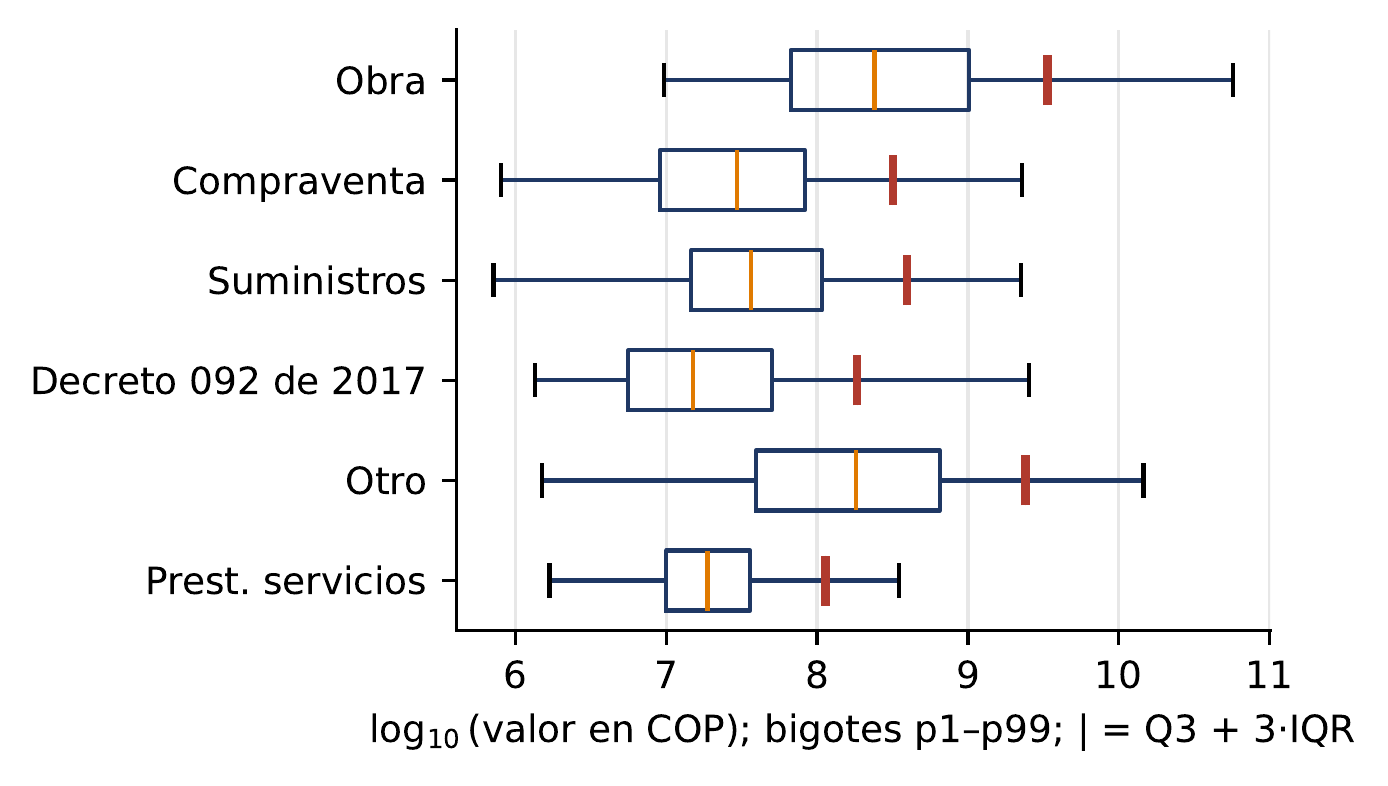
\includegraphics[width=\columnwidth]{figuras/fig_box_tipo.png}
\caption{Cómo se reparten los valores en cada tipo de contrato, sobre la muestra; la marca roja indica el límite de atípico obtenido con todos los datos.}
\label{mineria:fig:box}
\end{figure}

% =============================================================================
\subsection{Análisis exploratorio}
\label{mineria:sec:eda}
% =============================================================================
Los conteos salen exactos de las tablas de oro, y lo demás de una muestra de 51.570 contratos. La muestra se elige con un \emph{hash} del identificador, de modo que la misma consulta devuelve siempre los mismos contratos.

La contratación directa reúne el 76,6~\% de los contratos y apenas el 32,2~\% del valor, porque en su mayoría son prestaciones de servicios pequeñas, con una mediana de 18,7 millones de COP. Bogotá concentra el 32,9~\% de los contratos, y la proporción de contratación directa va del 75,7~\% allí al 90,1~\% en Valle del Cauca (Fig.~\ref{mineria:fig:departamentos}).

Se esperaba un pico en diciembre, pero cada año el mes con más contratos es enero o febrero (Fig.~\ref{mineria:fig:serie}). Los dos meses más altos de toda la serie son enero de 2022 y enero de 2026, ambos justo antes de una Ley de Garantías, y mientras dura la restricción la contratación directa pasa de más del 80~\% a menos del 20~\%. En la muestra, el 5,8~\% de los contratos se firmó en sábado o domingo y el plazo mediano es de 152 días. Fuera de la contratación directa las alertas son poco frecuentes (Tabla~\ref{adq:t7}), así que el análisis siguiente se fija en perfiles y combinaciones.

\begin{figure}[!htbp]
\centering



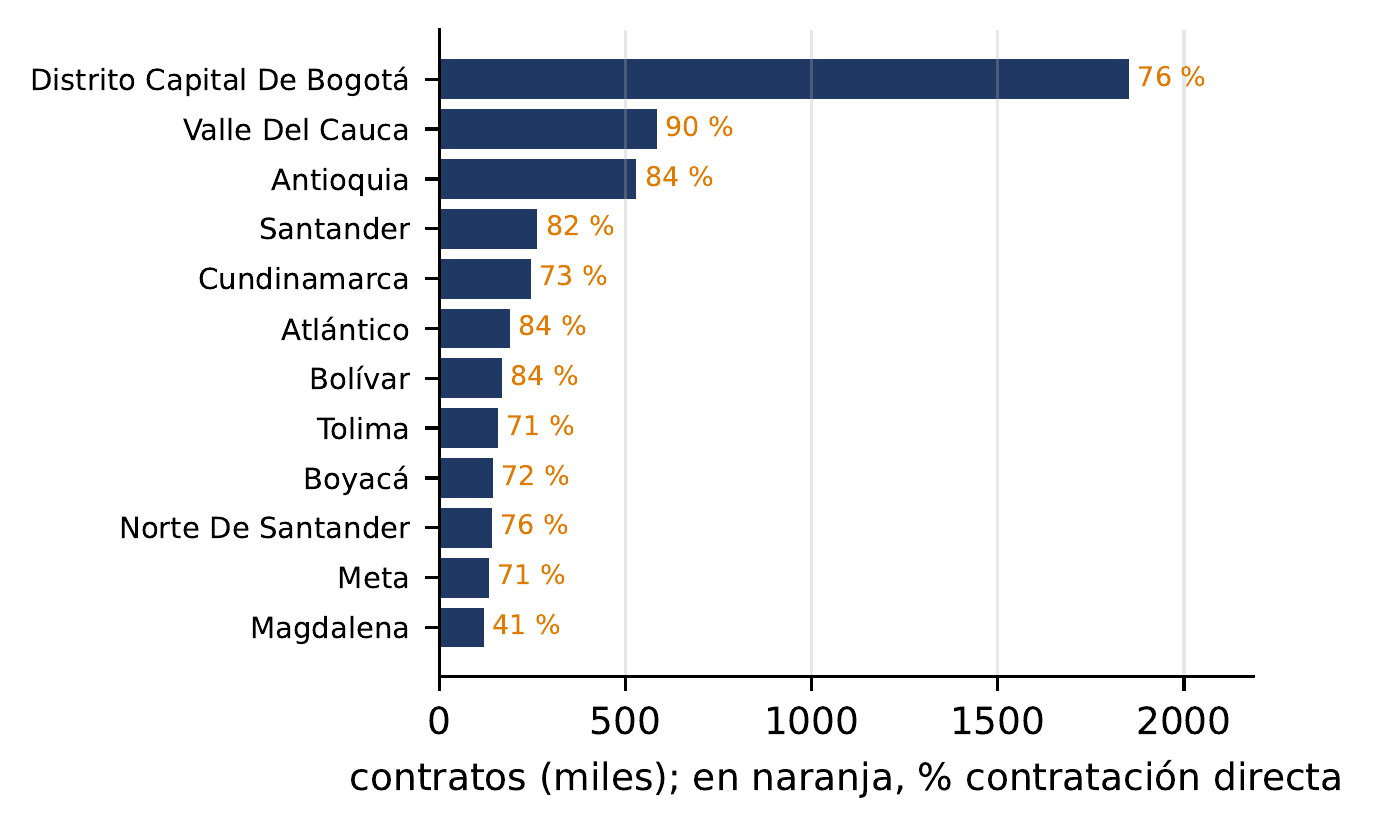
\includegraphics[width=\columnwidth]{figuras/fig_departamentos.png}
\caption{Doce departamentos con mayor número de contratos y la parte que se adjudica de forma directa.}
\label{mineria:fig:departamentos}
\end{figure}

\begin{figure}[!htbp]
\centering



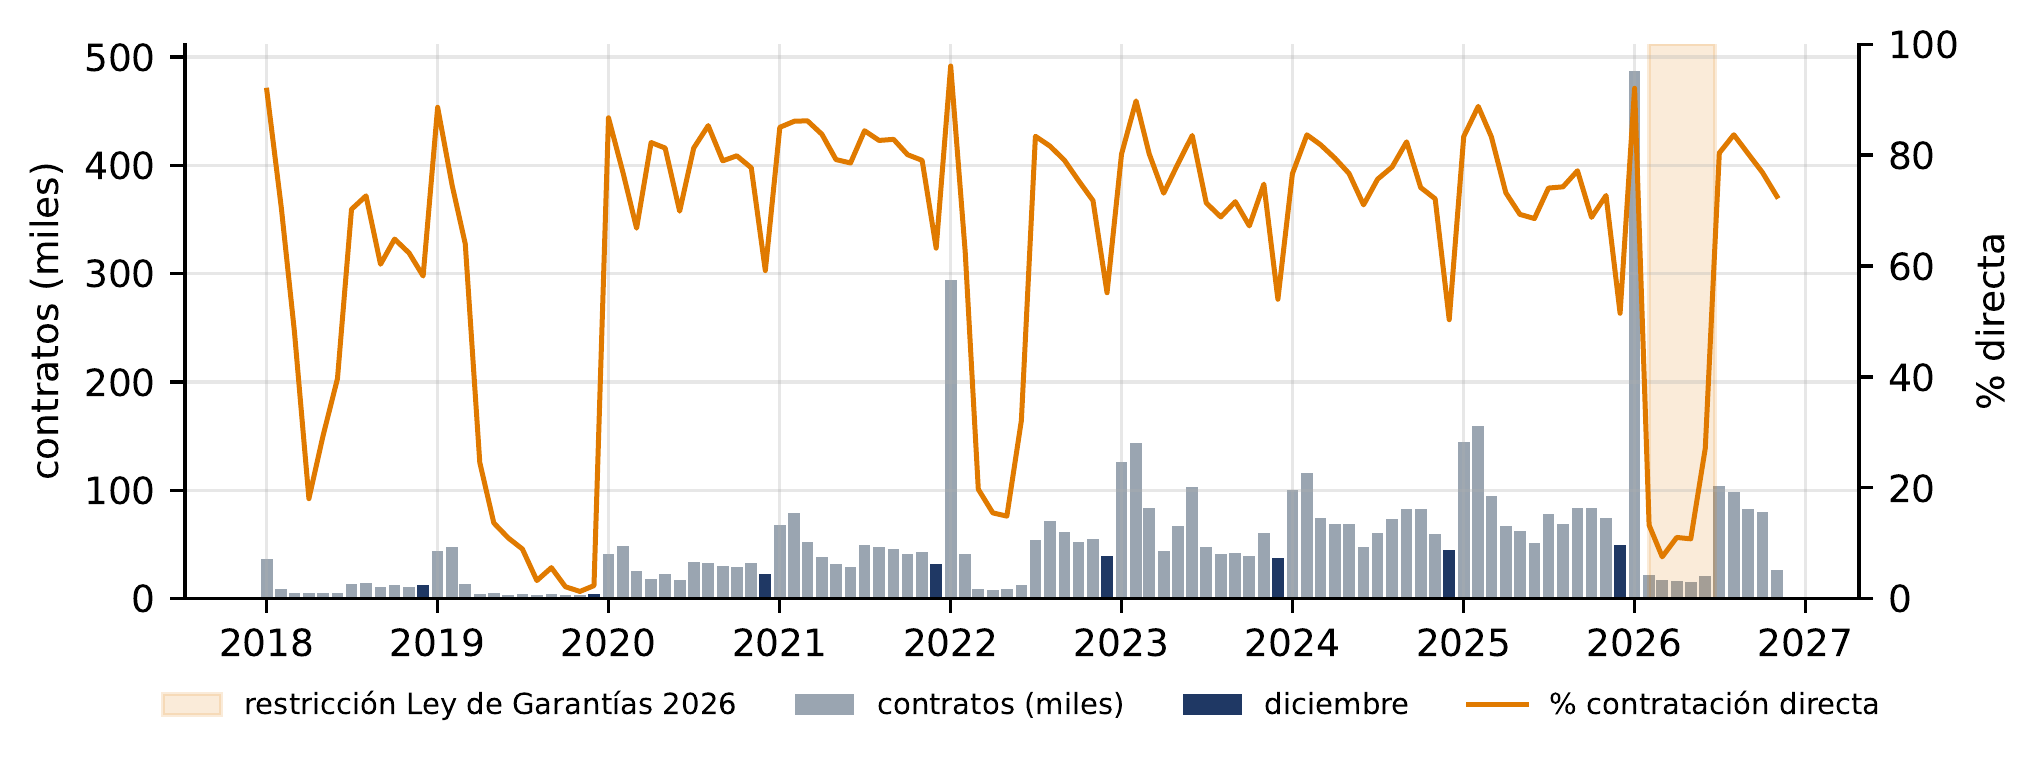
\includegraphics[width=\columnwidth]{figuras/fig_serie_mensual.png}
\caption{Contratos firmados mes a mes (barras, con diciembre destacado) y porcentaje adjudicado de forma directa (línea). En naranja, el periodo de restricción de 2026.}
\label{mineria:fig:serie}
\end{figure}

% =============================================================================
\subsection{Agrupamiento de entidades con K-means}
\label{mineria:sec:kmeans}
% =============================================================================
Se tomaron las 2.603 entidades con 20 contratos o más, que juntas suman el 99,8~\% de los contratos. Cada una se describe con ocho números: el porcentaje de sus contratos que activa cada una de siete alertas y la parte de su valor que se lleva su mayor contratista. El anticipo alto quedó fuera porque casi no varía entre entidades, y la alerta de concentración también, porque repite la participación del mayor contratista. A cada proporción se le sacó raíz cuadrada y luego se estandarizó, para que ninguna pese más que las otras en la distancia. El modelo es K-means~\cite{macqueen1967} con inicio k-means++~\cite{arthur2007}, en scikit-learn~\cite{pedregosa2011} y con semilla 42.

Para escoger $k$ se probaron valores de 2 a 10 y se compararon la inercia, la silhouette~\cite{rousseeuw1987} y el índice de Davies-Bouldin~\cite{davies1979} (Fig.~\ref{mineria:fig:codo}). De $k = 3$ en adelante, la mejor silhouette es la de $k=4$, con 0,213. Con $k=2$ los grupos solo separan a quienes contratan mucho o poco de forma directa, y eso no ayuda a priorizar. Al repetir el modelo con diez semillas, el índice de Rand ajustado~\cite{hubert1985} fue de 0,999, así que los grupos no dependen del azar. Una silhouette tan baja indica que los grupos se mezclan en los bordes y deben leerse como perfiles.

\begin{figure}[!htbp]
\centering



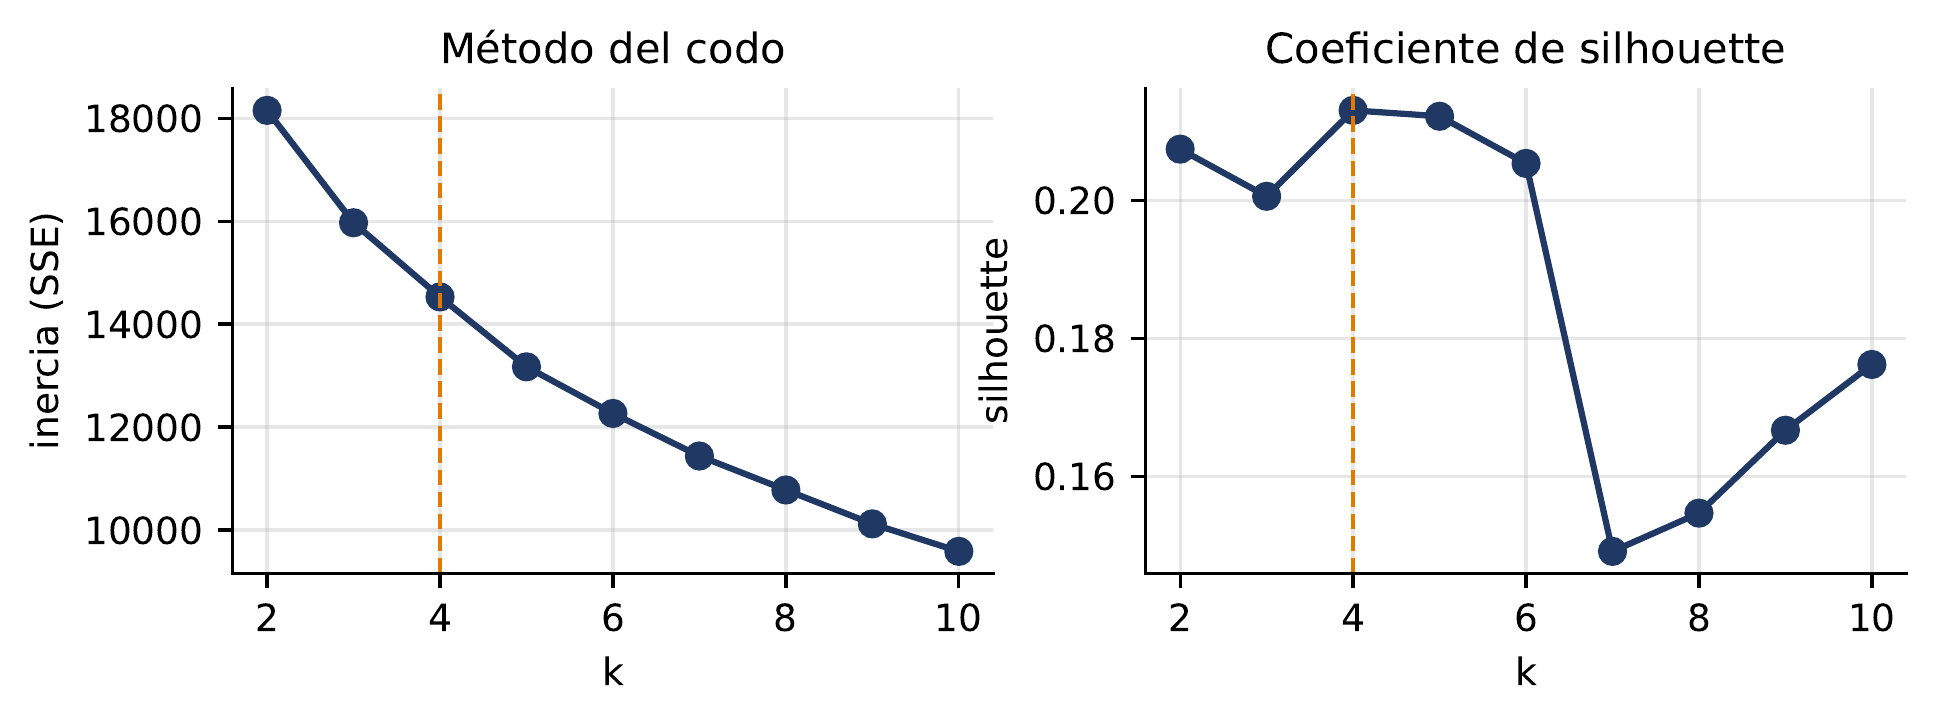
\includegraphics[width=\columnwidth]{figuras/fig_codo_silhouette.png}
\caption{Elección de $k$: inercia y silhouette. La línea naranja marca $k=4$.}
\label{mineria:fig:codo}
\end{figure}

La Fig.~\ref{mineria:fig:perfil} y la Tabla~\ref{mineria:tab:clusters} describen los cuatro grupos:
\begin{itemize}
  \item C1 reúne 541 entidades con pocas alertas y casi sin contratación directa. Muchas son hospitales públicos, que contratan por régimen especial.
  \item En las 304 entidades de C2, el 29~\% de los contratos empieza antes de firmarse, ocho veces el promedio nacional.
  \item En las 365 de C3, uno de cada cinco contratos supera el umbral de su tipo, y hay más adiciones y más contratistas sin identificar.
  \item C4 tiene 1.393 entidades que contratan de forma directa el 80,6~\% de las veces; ahí está el 77,8~\% de todos los contratos.
\end{itemize}

\begin{figure}[!htbp]
\centering



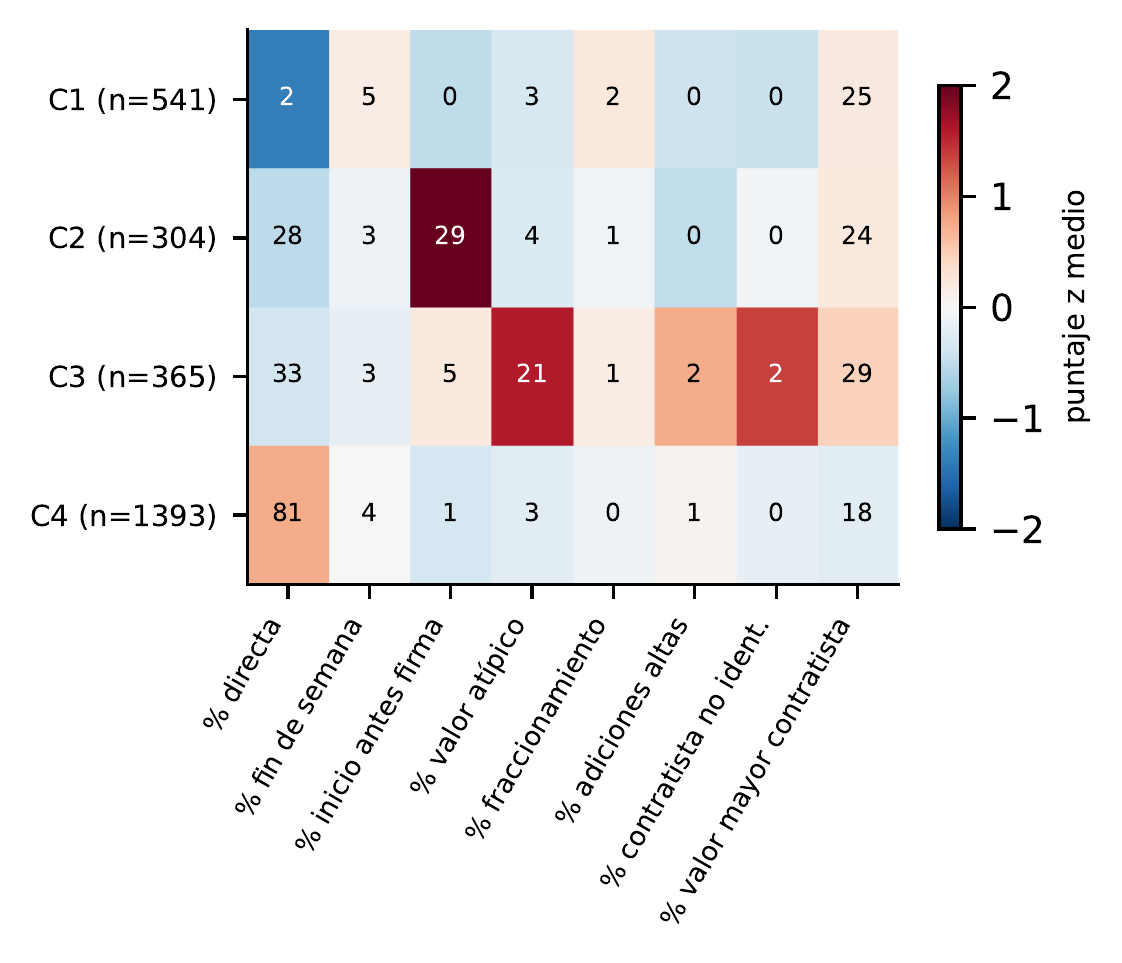
\includegraphics[width=\columnwidth]{figuras/fig_perfil_clusters.png}
\caption{Rasgos de cada grupo de entidades. El color muestra cuánto se aparta del promedio y la cifra, el porcentaje.}
\label{mineria:fig:perfil}
\end{figure}

\begin{table}[!htbp]
\centering
\caption{Promedios por entidad en cada uno de los cuatro grupos}
\label{mineria:tab:clusters}
\footnotesize
\begin{tabular}{@{}lrrrr@{}}
\toprule
 & C1 & C2 & C3 & C4 \\
\midrule
Entidades & 541 & 304 & 365 & 1.393 \\
Contratos (miles) & 381,5 & 292,3 & 590,4 & 4.426,5 \\
\% con una alerta o más & 13,5 & 55,8 & 58,9 & 83,7 \\
\% directa & 1,6 & 28,3 & 33,2 & 80,6 \\
\% inicio antes de firma & 0,3 & 29,0 & 4,8 & 0,8 \\
\% valor atípico & 3,1 & 3,5 & 21,1 & 2,6 \\
\% del principal proveedor & 24,6 & 24,3 & 29,3 & 17,8 \\
\bottomrule
\end{tabular}
\end{table}

Saber el grupo orienta la revisión: si la entidad está en C2, lo primero son las fechas; si está en C3, los montos y las prórrogas.

% =============================================================================
\subsection{Reglas de asociación entre alertas}
\label{mineria:sec:apriori}
% =============================================================================
Aquí cada contrato hace de transacción y cada alerta activa, de ítem. Athena agrupó los contratos según su combinación de alertas y encontró 129 combinaciones distintas con su número de contratos, de manera que el soporte se calcula exacto sobre todo el conjunto. Con Apriori~\cite{agrawal1994} y un soporte mínimo de 0,1~\% resultaron 21 conjuntos frecuentes y 30 reglas. La confianza y el lift de una regla $A\Rightarrow B$ son
\begin{equation}
\mathrm{conf}=\frac{\mathrm{sop}(A\cup B)}{\mathrm{sop}(A)},\qquad
\mathrm{lift}=\frac{\mathrm{conf}}{\mathrm{sop}(B)} ,
\end{equation}
y un lift por encima de 1 significa que las dos alertas coinciden más de lo que coincidirían por azar.

\begin{table}[!htbp]
\centering
\caption{Alertas que coinciden más (lift de 1,2 o más) y las que casi nunca van juntas}
\label{mineria:tab:reglas}
\footnotesize
\begin{tabular}{@{}lrrr@{}}
\toprule
Regla & Contratos & Conf. & Lift \\
\midrule
sin proveedor $\Rightarrow$ atípico & 7.170 & 44,2~\% & 10,62 \\
prórroga larga $\Rightarrow$ firmado en fin de semana & 9.846 & 14,0~\% & 2,41 \\
prórroga larga $\Rightarrow$ empezó sin firma & 6.089 & 8,7~\% & 2,36 \\
prórroga larga $\Rightarrow$ atípico & 6.251 & 8,9~\% & 2,14 \\
empezó sin firma $\Rightarrow$ atípico & 11.687 & 5,6~\% & 1,34 \\
\midrule
atípico $\Rightarrow$ adjudicación directa & 105.150 & 44,3~\% & 0,57 \\
prórroga larga $\Rightarrow$ adjudicación directa & 17.161 & 24,5~\% & 0,32 \\
\bottomrule
\end{tabular}
\end{table}

\begin{figure}[!htbp]
\centering



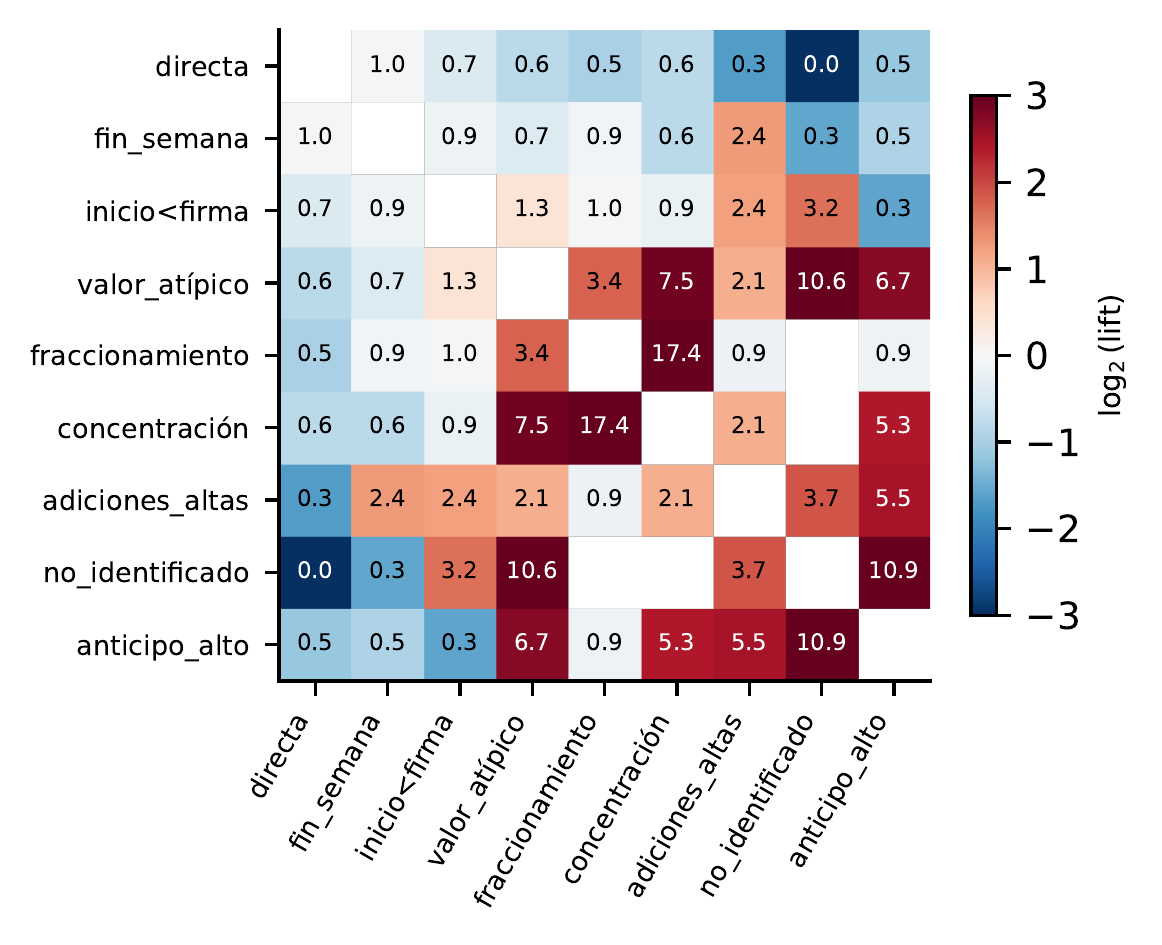
\includegraphics[width=\columnwidth]{figuras/fig_lift_pares.png}
\caption{Lift de cada par de alertas: en rojo coinciden más de lo que daría el azar y en azul, menos.}
\label{mineria:fig:lift}
\end{figure}

La relación más fuerte (Tabla~\ref{mineria:tab:reglas} y Fig.~\ref{mineria:fig:lift}) es entre no identificar al contratista y tener un valor atípico: el 44~\% de los contratos sin documento del contratista también es atípico, 10,6 veces lo esperado. Puede tratarse de contratos para revisar o de errores al publicar. Las adiciones altas suelen ir con firma en fin de semana, inicio antes de la firma y valores atípicos, lo que sugiere que los contratos mal planeados juntan varias alertas. La contratación directa, en cambio, tiene lift menor que 1 con casi todas las demás, y por eso no debería pesar tanto en el índice.

El código está en la carpeta \code{mineria/} del repositorio, con semilla fija y la misma muestra en cada corrida. Las nueve consultas leyeron 237~MB en Athena, lo que cuesta menos de un centavo de dólar~\cite{aws_athena_pricing}.

% =============================================================================
\subsection{Limitaciones}
% =============================================================================
Las alertas y los grupos señalan patrones y no dicen nada sobre la conducta de nadie, y como los grupos se mezclan en los bordes sirven para orientar la revisión, no para clasificar. Algunas entidades nacionales publican todo con un solo NIT aunque tengan sedes en varios departamentos, lo que distorsiona el análisis por territorio. Además, las cifras cambian con cada carga diaria; aquí se usa el corte del 13 de noviembre de 2026.

% =============================================================================
\subsection{Conclusiones}
% =============================================================================
\begin{itemize}
  \item Plata quedó limpia y sin duplicados, con los nulos sin rellenar y dos reglas distintas para los valores extremos.
  \item La exploración desmintió el supuesto pico de diciembre: el año arranca con la mayor contratación, en enero o febrero.
  \item K-means encontró cuatro perfiles de entidades que no cambian con la semilla, y Apriori mostró qué alertas se acompañan.
  \item Falta ponderar las alertas en el índice, probar métodos que manejen grupos mezclados, como DBSCAN o mezclas gaussianas, y revisar a mano una muestra de casos.
\end{itemize}
